\section{Experiment design}

\begin{figure}
	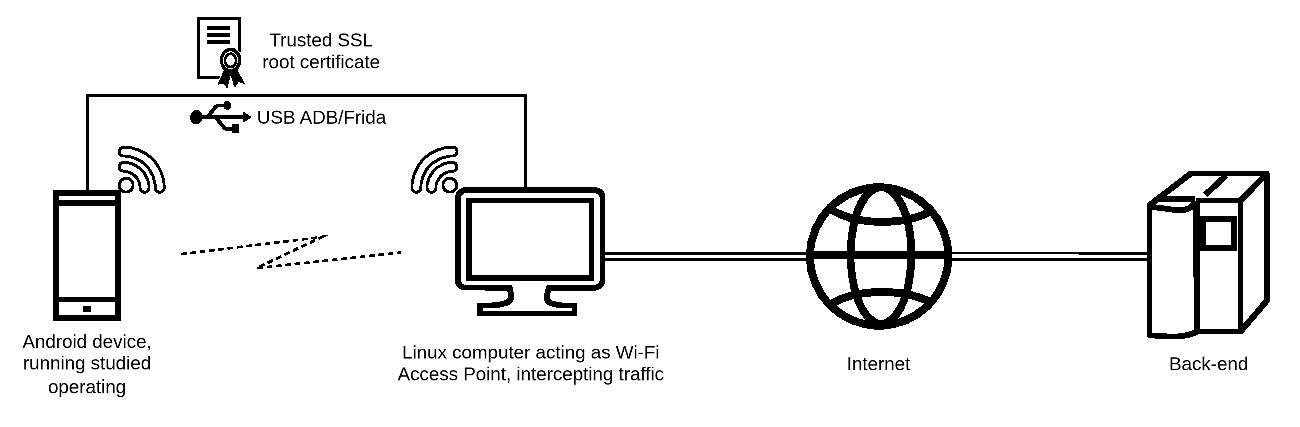
\includegraphics[width=\textwidth]{images/devices.eps}
	\caption{Measurement setup. Android device running studied operating systems is configured to access Internet using Wi-Fi. Access point is hosted on a Linux computer, running traffic interception and capturing software. Custom system certificate is installed on the phone using root access. USB connection is used for ADB/Frida communication.} \label{fig1}
\end{figure}

\subsection{Measurement Scenarios}
To enable consistent, comparable measurements across Android distributions, four setup scenarios were defined. Each scenario specifies (i) Google account state, (ii) consent/permission posture, and (iii) what Google components are present. Not all scenarios apply to every operating system due to their characteristics.

\paragraph{Scenario A: Default Setup with Google Account.}
The device is configured to reflect a typical user path. Google account sign-in is performed during setup (or immediately after) and default recommendations are accepted (including permissions).

\paragraph{Scenario A2: Minimal Setup with Google Account.}
This scenario applies exclusively to the official factory system. It extends \textit{Scenario A} by systematically minimizing privacy exposure while retaining Google account functionality. During and after initial setup, all optional consents and permissions are declined. System and account settings are adjusted to maximize user privacy. This scenario is not applicable to alternative distributions, as these systems are configured for privacy by default and do not implement or prompt users for privacy-threatening features characteristic of the factory system.

\paragraph{Scenario B: Minimal Setup without Google Account.}
The device is configured with maximum privacy in mind, avoiding Google account sign-in entirely. During initial setup, only strictly required prompts are accepted and optional data-sharing is declined. System settings are  adjusted to maximize user privacy. Google components or their functional replacements remain present and enabled to preserve baseline device functionality and app compatibility, but operate without account.

\paragraph{Scenario C: Extremely Minimal Setup without Google Components.}
This scenario applies only to distributions that do not bundle or enable Google components by default. The device is configured to operate without any Google Mobile Services, sandboxed Google Play, or microG. On GrapheneOS, this configuration is achieved by declining installation of Google components during initial setup; on LineageOS and iod\'eOS, microG is present but explicitly disabled. This scenario is not applicable to the official factory system, which bundles and enables Google components by default.

[Scenario adaptation to microg/graphene...]